\documentclass{article}
\usepackage{tikz}
\usetikzlibrary{arrows.meta}

\begin{document}

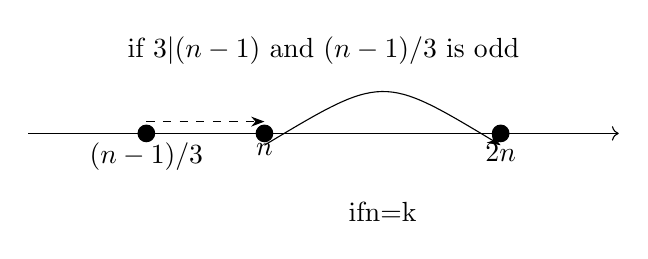
\begin{tikzpicture}[scale=1.5]
    % Draw the horizontal line
    \draw[->] (-2,0) -- (3,0);
    
    % Mark points on the line
    \filldraw[black] (-1,0) circle (2pt) node[below] {$(n-1)/3$};
    \filldraw[black] (0,0) circle (2pt) node[below] {$n$};
    \filldraw[black] (2,0) circle (2pt) node[below] {$2n$};
    
    % Dashed arrow from (n-1)/3 to n
    \draw[dashed, -Stealth] (-1,0.1) -- (0,0.1);
    
    % Text above the dashed arrow
    \node at (0.5, 0.5) [above] {if $3|(n-1)$ and $(n-1)/3$ is odd};
    
    % Curved arrow from n to 2n
    \draw[-Stealth] (0,-0.1) .. controls (1,0.5) .. (2,-0.1);
    
    % Text below the curved arrow
    \node at (1,-0.5) [below] {if \\ n=k};
\end{tikzpicture}

\end{document}